\section{Downstream cosmology module on the observation-closed branch}
\label{sec:cosmology-closure}

\begin{lemma}[Automatic seam-transfer convergence]
\label{lem:automatic-seam-transfer-convergence}
On the admissible branch the seam transfer operator
\[
\mathcal U_\Seam:=\Padm e^{-\ell_\Seam|B_\Seam|}\Padm
\]
is positive and trace class. Moreover,
\[
0<\mathcal U_\Seam\le e^{-S_\Seam}\Padm,
\qquad
S_\Seam:=\ell_\Seam\lambda_1^+(B_\Seam)>0.
\]
Hence
\[
\mathrm{Spec}(\mathcal U_\Seam)\subset (0,e^{-S_\Seam}] \subset (0,1),
\]
so the Fredholm determinant
\[
-\log\det_{\mathrm{adm}}(1-\mathcal U_\Seam)
\]
converges absolutely and defines a positive quantity.
\end{lemma}

\begin{proposition}[Downstream cosmology module on the observation-closed branch]
\label{thm:cosmology-closure}
On the numerically selected observation-closed branch, the following cosmology-facing quantities
are evaluated from the same retained operator data and comparison choices:
\begin{enumerate}[label=(\roman*), leftmargin=1.5em, topsep=3pt, itemsep=2pt]
    \item the scalaron reheating temperature is fixed by the scalaron width derived from the
    $R^2$ branch,
    \[
    T_R=
    \left(\frac{90}{\pi^2 g_\ast}\right)^{1/4}
    \sqrt{\Gamma_\varphi \Mplunred},
    \]
    \item the PQ branch is closed by
    \[
    N_{\mathrm{DW}}=1,
    \qquad
    \theta_i=\pi(1-\phiz),
    \qquad
    \Omega_a h^2=
    \Delta_R^{-1}
    \bigl[
    \Omega_a^{\mathrm{mis}}(f_a,m_a,\theta_i)
    +
    \Omega_a^{\mathrm{str}}(f_a,N_{\mathrm{DW}})
    \bigr],
    \]
    \item the baryon asymmetry is fixed by flavored leptogenesis on the same neutrino branch,
    \[
    \eta_B=c_{\mathrm{sph}}\sum_\alpha \kappa_\alpha\,\varepsilon_{1\alpha},
    \]
    \item and the observed cosmological constant is generated by the positive trace-class seam
    transfer operator
    \[
    \mathcal U_\Seam:=\Padm e^{-\ell_\Seam |B_\Seam|}\Padm,
    \qquad
    \ell_\Seam\,\lambda_1^+(B_\Seam)=S_\Seam,
    \qquad
    S_\Seam:=\frac{2\pi}{3}\alpha^{-1}(0),
    \]
    through
    \[
    \Lambda_{\mathrm{obs}}
    =
    \Mplunred^4
    \Bigl[-\log\det\nolimits_{\mathrm{adm}}(1-\mathcal U_\Seam)\Bigr].
    \]
\end{enumerate}
By \Cref{lem:automatic-seam-transfer-convergence}, the determinant expansion converges
absolutely and yields a positive cosmological constant on the selected branch. This subsection
records a downstream module rather than a standalone closure theorem on the core theorem surface.
\end{proposition}

\begin{remark}[Minimal dark-sector reading on the canonical branch]
On the minimal branch the dominant dark-matter component is axionic and the only irreducible
hot dark component is the neutrino background. No extra dark sector is required for closure.
\end{remark}

Appendix-level E$_8$ arithmetic continuations and asymptotic scale-grammar formulas are collected
in Appendix~\ref{app:constants} and are not part of the main theorem surface.

\section{Primary benchmark map and prediction ledger}

The comparison values used in this section follow representative CODATA, PDG, NuFIT, Planck,
and birefringence references
\cite{codata2022,pdg2025,nufit2025,planck2018,minamiKomatsu2020,eskilt2023,sullivan2025}. The
snapshot policy is frozen at CODATA 2022 / NIST for $\alpha(0)$, PDG 2025 for particle-mass and
weak-mixing rows, NuFIT 2025 for neutrino-angle rows, and Planck 2018 for the baryon-fraction
reconstruction used here. The main-text table is intentionally restricted to six rows whose
comparison language is already convention-complete under the intrinsic observation functor. The
compact mass surface is given separately in
\Cref{tab:sm-mass-ledger-ew,tab:sm-mass-ledger-quarks}; more exploratory rows are moved to
Appendix~\ref{app:benchmarks}. Beyond that narrow six-row surface, the manuscript also carries a
small operational prediction set of experimentally actionable rows, collected explicitly below.
The $\Omega_b$ row is a present-epoch reconstruction from the Planck pair $(\Omega_b h^2,H_0)$,
not a claim that $\Omega_b(t)$ itself is a timeless seed quantity. Here \enquote{carrier
closure} abbreviates the exact electromagnetic closure equation built from the exact seam
generating function $\phiseam(\alpha)$. The $\alpha^{-1}(0)$ row is therefore structurally
different from the four seed-driven observation rows
$(\beta,\Omega_b,\lambda_C,\sin^2\theta_{13})$, which are all projections of the same canonical
seed $\phiz$.

\begin{table}[t]
\centering
\scriptsize
\setlength{\tabcolsep}{2pt}
\resizebox{\linewidth}{!}{%
\begin{tabular}{@{}llrrrrll@{}}
\toprule
\makecell[l]{Obs.} & \makecell[l]{TFPT\\formula} & \makecell[r]{TFPT\\value} & \makecell[r]{Exp.\\value} & \makecell[r]{Unc.} & \makecell[r]{Residual} & \makecell[l]{Scale /\\scheme} & Status \\
\midrule
$\alpha^{-1}(0)$ & \makecell[l]{exact electromagnetic closure\\$\phiseam(\alpha)$} & \num{137.0359992} & \num{137.03599918} & \num{2.1e-8} & $+1.87\sigma$ & \makecell[l]{Thomson\\on-shell} & exact algebraic \\
\makecell[l]{$\bar\alpha^{(5)}$\\$(M_Z)^{-1}$} & \makecell[l]{$\mathcal R_{\SM}$\\$[\alpha(0)]$} & \num{127.9405} & \num{127.93} & \num{0.008} & $+1.32\sigma$ & \makecell[l]{$\overline{\mathrm{MS}}$\\at $M_Z$} & matched intrinsic observation \\
$\lambda_C$ & $\sqrt{\phiz(1-\phiz)}$ & \num{0.22438} & \num{0.22431} & \num{8.5e-4} & $+0.08\sigma$ & \makecell[l]{CKM\\proxy} & matched intrinsic observation \\
$\sin^2\theta_{13}$ & \makecell[l]{$\phiz$\\$e^{-5/6}$} & \num{0.02311} & \num{0.02224} & \num{5.7e-4} & $+1.524\sigma$ & \makecell[l]{NuFIT\\NO} & matched intrinsic observation \\
$\Omega_b$ & \makecell[l]{$(4\pi-1)$\\$\beta_{\mathrm{rad}}$} & \num{0.04894} & \num{0.04930} & \num{8.57e-4} & $-0.421\sigma$ & \makecell[l]{Planck 2018\\present epoch\\from $\Omega_b h^2$} & matched intrinsic observation \\
$\beta$ & \makecell[l]{$\beta_{\mathrm{rad}}$\\in degrees} & \num{0.242} & \num{0.35} & \num{0.14} & $-0.77\sigma$ & \makecell[l]{Planck 2018\\Minami--Komatsu} & matched intrinsic observation \\
\bottomrule
\end{tabular}}
\caption{Primary main-text benchmark table. The $\alpha^{-1}(0)$ row is exact algebraic, while the remaining rows are matched intrinsic observation images, with $(\beta,\Omega_b,\lambda_C,\sin^2\theta_{13})$ forming one seed-driven dependency cluster. Supplementary rows and out-of-sample checks are collected in Appendix~\ref{app:benchmarks}.}
\label{tab:benchmark}
\end{table}

\begin{remark}[One seed, four observation projections]
The seed-driven observation rows are not statistically independent hits. With
\[
\beta_{\mathrm{rad}}=\frac{\phiz}{4\pi},
\qquad
\Omega_b=(4\pi-1)\beta_{\mathrm{rad}},
\qquad
\lambda_C=\sqrt{\phiz(1-\phiz)},
\qquad
\sin^2\theta_{13}=\phiz e^{-\gamma},
\]
the four-row map is a one-variable seed map
\[
\mathcal S(\phiz):=\bigl(\beta_{\mathrm{rad}},\Omega_b,\lambda_C,\sin^2\theta_{13}\bigr),
\]
with Jacobian
\[
\frac{d\mathcal S}{d\phiz}
=
\left(
\frac{1}{4\pi},
\,
1-\frac{1}{4\pi},
\,
\frac{1-2\phiz}{2\sqrt{\phiz(1-\phiz)}},
\,
e^{-\gamma}
\right).
\]
Thus $\beta$, $\Omega_b$, $\lambda_C$, and $\sin^2\theta_{13}$ are one seed and four shadows,
not four detached observation events. They remain in the table because their comparison
conventions and uncertainty models differ, not because the underlying algebraic source is
independent.
\end{remark}

\subsection{Operational prediction set}

The six-row observation table is not the whole experimental surface of the manuscript.
\Cref{tab:operational-prediction-set} collects the rows that are operationally testable on near-
to medium-term timescales, while keeping their status, next test, kill criterion, and dependency
structure explicit. The point is not to flatten them into one truth class. Rather, the
\emph{Status} column now uses only the manuscript's final output vocabulary, and the derivation
and dependency columns show which rows are direct theorem outputs and which are intrinsic
observation images under $\mathcal R_{\mathrm{TOE}}$. The electroweak triple
$(m_W,\hat s_Z^2,\alpha_s)$ is omitted here only for compactness; by
\Cref{thm:observation-closure,cor:intrinsic-threshold-outputs} these rows already belong to the
intrinsic observation layer.

\begin{table}[t]
\centering
\tiny
\sisetup{round-mode=none, group-minimum-digits=20}
\setlength{\tabcolsep}{0.8pt}
\renewcommand{\arraystretch}{0.95}
\sloppy
\resizebox{\linewidth}{!}{%
\begin{tabular}{@{}>{\raggedright\arraybackslash}p{0.12\linewidth}>{\raggedright\arraybackslash}p{0.17\linewidth}>{\raggedright\arraybackslash}p{0.09\linewidth}>{\raggedright\arraybackslash}p{0.13\linewidth}>{\raggedright\arraybackslash}p{0.12\linewidth}>{\raggedright\arraybackslash}p{0.17\linewidth}>{\raggedright\arraybackslash}p{0.11\linewidth}@{}}
\toprule
\makecell[l]{Observable} & \makecell[l]{TFPT\\target} & Status & \makecell[l]{Derivation\\source} & \makecell[l]{Next\\test} & \makecell[l]{Kill\\criterion} & \makecell[l]{Dependency\\class} \\
\midrule
\makecell[l]{Cosmic\\birefringence $\beta$} & \num{0.2424}$^\circ$ & \makecell[l]{Matched intrinsic\\observation} & seed map $\beta=\phiz/(4\pi)$ & \makecell[l]{calibrated CMB\\rotation analysis} & \makecell[l]{calibrated $\beta=0$\\within $\pm \num{0.05}^\circ$} & seed \\
$\delta_{\mathrm{CKM}}$ & \makecell[l]{\num{1.198}\\rad} & \makecell[l]{Matched intrinsic\\observation} & \makecell[l]{exact holonomy\\phase / phase lattice} & \makecell[l]{global flavor\\fit} & \makecell[l]{exclusion at\\$\ge 3\sigma$} & \makecell[l]{flavor\\observation} \\
\makecell[l]{Rare kaons\\$K\to\pi\nu\bar\nu$} & \makecell[l]{$\mathrm{BR}(K^+)$\\$=\num{9.40e-11}$\\$\mathrm{BR}(K_L)$\\$=\num{3.47e-11}$} & \makecell[l]{Matched intrinsic\\observation} & \makecell[l]{exact CKM point in\\short-distance\\amplitudes} & \makecell[l]{NA62 / KOTO\\program} & \makecell[l]{$K^+$ outside\\$[7,12]\times10^{-11}$\\or $K_L$ mismatch} & \makecell[l]{flavor\\observation} \\
\makecell[l]{PMNS phase /\\octant} & \makecell[l]{$\delta_{\mathrm{CP}}=240^\circ$\\$\sin^2\theta_{23}=\num{0.4557}$} & \makecell[l]{Matched intrinsic\\observation} & \makecell[l]{neutrino closure /\\phase lattice} & \makecell[l]{global oscillation\\fit} & \makecell[l]{exclude $240^\circ$\\or lower octant\\at $\ge 3\sigma$} & \makecell[l]{neutrino\\observation} \\
$\Sigma m_\nu$ & \makecell[l]{\num{5.8764e-2}\\eV} & \makecell[l]{Matched intrinsic\\observation} & \makecell[l]{neutrino closure\\(NO)} & \makecell[l]{cosmological\\mass-sum analyses} & \makecell[l]{robust upper bound\\below the branch value} & \makecell[l]{neutrino\\observation} \\
$m_{\beta\beta}$ & \makecell[l]{\num{1.516e-3}\\eV} & \makecell[l]{Matched intrinsic\\observation} & \makecell[l]{Majorana lattice\\on the closed\\neutrino branch} & \makecell[l]{light-Majorana\\$0\nu\beta\beta$ searches} & \makecell[l]{detection implying\\$m_{\beta\beta}\gtrsim \num{1e-2}$ eV} & \makecell[l]{neutrino\\observation} \\
\makecell[l]{nEDM / strong\\CP} & $\bar\theta=0$ & \makecell[l]{Conditional\\closure} & \makecell[l]{admissibility-side\\strong-CP theorem} & \makecell[l]{next-gen EDM\\searches} & \makecell[l]{stable nonzero\\hadronic EDM signal} & closure \\
\makecell[l]{Axion haloscope\\window} & \makecell[l]{$m_a\approx \num{65.19}$\\$\mu\mathrm{eV}$\\$\nu_a\approx \num{15.764}$\\$\mathrm{GHz}$} & \makecell[l]{Optional\\extrapolation} & \makecell[l]{PQ block /\\downstream cosmology module} & \makecell[l]{haloscope scan\\near \num{15.764} GHz} & \makecell[l]{exclusion in\\\num{15.764} GHz\\$\pm \num{50}$ MHz} & \makecell[l]{cosmology\\observation} \\
\bottomrule
\end{tabular}}
\caption{Operational prediction set with explicit status and dependency classes.}
\label{tab:operational-prediction-set}
\end{table}

\begin{remark}[Independence classes]
The rightmost column in \Cref{tab:operational-prediction-set} records dependency structure
rather than truth value, using deliberately compact class labels. \emph{Seed} means a row is a
projection of the canonical scalar seed $\phiz$; \emph{flavor observation} means it is
downstream of the exact CKM transport output under $\mathcal R_{\mathrm{TOE}}$; \emph{neutrino
observation} means it belongs to the closed neutrino branch after observation matching;
\emph{closure} means it is a direct consequence of an admissibility-closure theorem; and
\emph{cosmology observation} means it is generated by the downstream cosmology module and then
read on the observation layer. This keeps statistical and logical non-independence visible at the same place
where the experimental targets are listed.
\end{remark}

\subsection{Compact prediction ledger}

The main observation table shows only a narrow comparison surface. To keep the compiler
structure visible, \Cref{tab:prediction-ledger} summarizes which output packages belong to which
layer of the paper.

\begin{table}[t]
\centering
\small
\begin{tabularx}{\linewidth}{@{}>{\raggedright\arraybackslash}p{0.18\linewidth}>{\raggedright\arraybackslash}p{0.12\linewidth}YY@{}}
\toprule
Domain & Status & Output package & Source layer \\
\midrule
Carrier packet & Exact algebraic & $E_3\oplus E_2$, $G_{\SM}^{\mathrm{glob}}$, $S^+$, $\gamma$, $\bone(N_{\mathrm{fam}},N_\Phi)$ & minimal carrier theorem and half-spinor decomposition \\
Kernel constants & Exact algebraic & $\cthree$, $\phibase$, $\phiz$, $\deltatop$ & exact seam opening and carrier-form closure equation \\
Family / occupancy layer & Conditional geometric or closure & $\Padm$, $F$, $\Oadm=48$, $\deltatop$ & topological family theorem, admissibility complex, and occupancy corollary \\
Geometric compiler & Conditional geometric or closure & $\Phi$, $\Mpl$, $\vgeo$, $R^2$ channel & bosonic index plus Dirac-anchor heat-kernel closure \\
Transport compiler & Conditional geometric or closure & $Y_f$, $m_f$, CKM, PMNS & transport-branch program and exact family-holonomy phase theorem \\
QCD closure & Conditional geometric or closure & $\Hhad$, anomaly inflow, $\bar\theta=0$ & singlet admissibility plus positive-kernel hardening \\
Observation layer & Matched intrinsic observation & $\mathcal R_{\mathrm{TOE}}$, $\alpha$, $\beta$, $\lambda_C$, threshold rows, ledgers & conditional closure-selection theorem with scheme-covariant numerical preconditioner $\mathcal R_{\SM}$ \\
Cosmology block & Optional extrapolation & $\Omega_{\mathrm{DM}}$, $\eta_B$, $\Lambda_{\mathrm{obs}}$, axion window & downstream cosmology module on the selected branch \\
Record layer & Conditional geometric or closure & $\Arec$, $\Aobs$, $\Pred$ & admissible gap plus observer-algebra definition \\
Optional extrapolation & Optional extrapolation & E$_8$ scale ratios and modular inner-seam language & appendix-level scale grammar and horizon extension \\
\bottomrule
\end{tabularx}
\caption{Compact prediction ledger for the carrier-first compiler presentation after the main-text
surface is split into exact algebraic outputs, conditional closure statements, matched intrinsic observation rows, and optional extrapolations.}
\label{tab:prediction-ledger}
\end{table}

\subsection{Realism audit of the present compiler surface}

The present main-text surface is no longer intentionally mixed. Its rows now use the manuscript's
four final classes: exact algebraic, conditional geometric or closure, matched intrinsic
observation, and optional extrapolation. Carrier algebra and the exact $\alpha$ row remain the
sharpest numerically load-bearing entries, while the seed-driven observation rows remain useful
because they are transparent and mutually constrained rather than statistically independent. The
transport block is now generative up to observation matching, the neutrino block is read on the
same selected branch, and the electroweak threshold rows are matched intrinsic observations.
What remains outside this main-text surface is optional extrapolation, not unresolved theorem
load hidden in the core.

\subsection{Residual map and principal comparison refinements}

The residuals for the restricted six-row observation table are shown in
\Cref{fig:residual-plot}. The carrier-linked electromagnetic, birefringence, and baryon-density
channels all remain within the displayed few-sigma window. The CKM phase is not plotted here
because it is better treated in the operational prediction set and Appendix~\ref{app:benchmarks}
rather than inside the restricted six-row residual plot.

\begin{figure}[t]
\centering
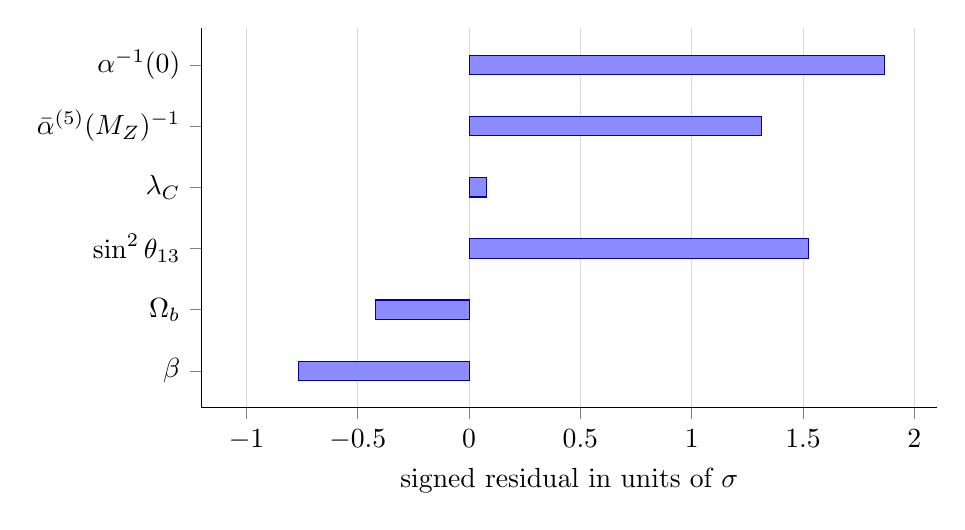
\begin{tikzpicture}
\begin{axis}[
    width=0.9\linewidth,
    height=6.4cm,
    xbar,
    bar width=7pt,
    xmin=-1.2,
    xmax=2.1,
    xlabel={signed residual in units of $\sigma$},
    symbolic y coords={beta,omegab,theta13,lambdac,alphaMZ,alpha0},
    ytick=data,
    yticklabels={$\beta$,$\Omega_b$,$\sin^2\theta_{13}$,$\lambda_C$,$\bar\alpha^{(5)}(M_Z)^{-1}$,$\alpha^{-1}(0)$},
    enlarge y limits=0.12,
    axis x line*=bottom,
    axis y line*=left,
    tick align=outside,
    major grid style={draw=gray!30},
    xmajorgrids=true
]
\addplot[fill=blue!45, draw=blue!70!black] coordinates {
    (-0.768,beta)
    (-0.421,omegab)
    (1.524,theta13)
    (0.078,lambdac)
    (1.315,alphaMZ)
    (1.865,alpha0)
};
\end{axis}
\end{tikzpicture}
\caption{Residual plot for the main intrinsic-observation rows with declared uncertainties.}
\label{fig:residual-plot}
\end{figure}

The principal remaining refinements are therefore specific rather than diffuse:
\begin{itemize}[leftmargin=1.5em, topsep=3pt, itemsep=2pt]
    \item the CKM phase is read from the exact holonomy phase, with only the small-area transport asymptotic kept as a derived expansion,
    \item the nonabelian comparison channels now split into fixed local carrier closure and explicit matching functionals, so the remaining sensitivity is numerical rather than structural,
    \item direct-search interface rows remain pressure tests on the closed branch rather than precision residual rows.
\end{itemize}

\subsection{Falsification matrix}

The present draft does not ask the reader to accept one undifferentiated \enquote{compiler} claim. Each main-text closure statement has a corresponding local or global failure mode, and those failure modes should be readable without first decoding the appendix tables.

The matrix below is therefore intentionally short. It collects only the load-bearing main-paper statements whose failure would break the carrier-first architecture at the theorem level, rather than every downstream benchmark row or optional appendix interface.

\begin{table}[t]
\centering
\small
\begin{tabularx}{\linewidth}{@{}>{\raggedright\arraybackslash}p{0.24\linewidth}YY>{\raggedright\arraybackslash}p{0.13\linewidth}@{}}
\toprule
Statement & What would falsify it & Sector affected & Local or global failure \\
\midrule
Primitive relative spectral dynamics & ill-posed APS domain or no finite admissible spectral action on the retained branch & Hard / closure & global \\
Minimal carrier $E_3\oplus E_2$ & failure to recover the one-family packet or the global quotient from the carrier theorem & Hard & global \\
Topological family closure and $\Oadm=48$ & failure of the topological family theorem to globalize the local count & Closure & local-to-structural \\
Bosonic relative index selecting $\Phi$ & no unique seam-even doublet or an unavoidable extra light triplet & Closure & local \\
local spectral-scale / gravity closure for $\Mpl$ and $\vgeo$ & inability to obtain one common closure for $\Mpl$, $\vgeo$, the Einstein branch, and the $R^2$ branch & Closure & global \\
Transport / strong-CP closure & nonzero determinant phase or an unavoidable $\bar\theta$ counterterm & Closure & local \\
Confinement as admissible word selection & necessity of physical states with $z(w)\neq1$ in the low-energy spectrum & Closure & local \\
Nonperturbative admissible QFT closure & no admissible mass gap or no clustering on the retained branch & Closure & global \\
\bottomrule
\end{tabularx}
\caption{Falsification matrix for the present main-paper claims.}
\label{tab:falsification}
\end{table}

\section{Compiler theorem and intrinsic observation}

\subsection{Compiler chain}

Collecting the admissible reduced datum, primitive reconstruction, the closure theorems from the
admissibility complex, and the intrinsic observation layer, the compiler line is
\begin{equation}
\label{eq:closed-compiler-chain}
\begin{aligned}
\Tmin^{\mathrm{adm}}
&\Rightarrow
\Tprim^{\mathrm{kin}}\\
&\Rightarrow
(E_3\oplus E_2,\ G_{\SM}^{\mathrm{glob}},\ S^+)\\
&\Rightarrow
(\Padm,\ F,\ \Oadm=48,\ \Phi,\ \Mpl,\ \vgeo,\ \nabla_F^\star)\\
&\Rightarrow
x_{\mathrm{core}}^\star\\
&\Rightarrow
\mathcal R_{\mathrm{TOE}}
\;\Rightarrow\;
O_{\mathrm{th}}.
\end{aligned}
\end{equation}
This line is not meant as a slogan. Each arrow is attached either to a hard theorem or to one of
the closure theorems of \Cref{sec:closure-theorems}. In practical finite-threshold computations,
$\mathcal R_{\SM}$ is only the numerical preconditioner used to approximate
$\mathcal R_{\mathrm{TOE}}$.

